%%% Hlavní soubor. Zde se definují základní parametry a odkazuje se na ostatní části. %%%

%% Verze pro jednostranný tisk:
% Okraje: levý 40mm, pravý 25mm, horní a dolní 25mm
% (ale pozor, LaTeX si sám přidává 1in)
\documentclass[12pt,a4paper]{report}
\setlength\textwidth{145mm}
\setlength\textheight{247mm}
\setlength\oddsidemargin{15mm}
\setlength\evensidemargin{15mm}
\setlength\topmargin{0mm}
\setlength\headsep{0mm}
\setlength\headheight{0mm}
% \openright zařídí, aby následující text začínal na pravé straně knihy
\let\openright=\clearpage

%% Pokud tiskneme oboustranně:
% \documentclass[12pt,a4paper,twoside,openright]{report}
% \setlength\textwidth{145mm}
% \setlength\textheight{247mm}
% \setlength\oddsidemargin{15mm}
% \setlength\evensidemargin{0mm}
% \setlength\topmargin{0mm}
% \setlength\headsep{0mm}
% \setlength\headheight{0mm}
% \let\openright=\cleardoublepage

%% Pokud používáte csLaTeX (doporučeno):
\usepackage{czech}
%% Pokud nikoliv:
%\usepackage[czech]{babel}
%\usepackage[T1]{fontenc}

%% Použité kódování znaků: obvykle latin2, cp1250 nebo utf8:
\usepackage[utf8]{inputenc}

%% Ostatní balíčky
\usepackage{graphicx}
\usepackage{amsthm}

%% Balíček hyperref, kterým jdou vyrábět klikací odkazy v PDF,
%% ale hlavně ho používáme k uložení metadat do PDF (včetně obsahu).
%% POZOR, nezapomeňte vyplnit jméno práce a autora.
\usepackage[ps2pdf,unicode]{hyperref}   % Musí být za všemi ostatními balíčky
\hypersetup{pdftitle=Hledání pěších cest v mapě}
\hypersetup{pdfauthor=Tomáš Pokorný}

%%% Drobné úpravy stylu

% Tato makra přesvědčují mírně ošklivým trikem LaTeX, aby hlavičky kapitol
% sázel příčetněji a nevynechával nad nimi spoustu místa. Směle ignorujte.
\makeatletter
\def\@makechapterhead#1{
  {\parindent \z@ \raggedright \normalfont
   \Huge\bfseries \thechapter. #1
   \par\nobreak
   \vskip 20\p@
}}
\def\@makeschapterhead#1{
  {\parindent \z@ \raggedright \normalfont
   \Huge\bfseries #1
   \par\nobreak
   \vskip 20\p@
}}
\makeatother

% Toto makro definuje kapitolu, která není očíslovaná, ale je uvedena v obsahu.
\def\chapwithtoc#1{
\chapter*{#1}
\addcontentsline{toc}{chapter}{#1}
}

\begin{document}

% Trochu volnější nastavení dělení slov, než je default.
\lefthyphenmin=2
\righthyphenmin=2

%%% Titulní strana práce

\pagestyle{empty}
\begin{center}

\large

Univerzita Karlova v Praze

\medskip

Matematicko-fyzikální fakulta

\vfill

{\bf\Large BAKALÁŘSKÁ PRÁCE}

\vfill

\centerline{\mbox{
\includegraphics[width=60mm]{../img/logo.eps}}}

\vfill
\vspace{5mm}

{\LARGE Tomáš Pokorný}

\vspace{15mm}

% Název práce přesně podle zadání
{\LARGE\bfseries Hledání pěších cest v mapě}

\vfill

% Název katedry nebo ústavu, kde byla práce oficiálně zadána
% (dle Organizační struktury MFF UK)
Katedra aplikované matematiky

\vfill

\begin{tabular}{rl}

Vedoucí bakalářské práce: & Mgr. Martin Mareš, Ph.D. \\
\noalign{\vspace{2mm}}
Studijní program: & Informatika \\
\noalign{\vspace{2mm}}
Studijní obor: & Obecná informatika \\
\end{tabular}

\vfill

% Zde doplňte rok
Praha 2014

\end{center}

\newpage

%%% Následuje vevázaný list -- kopie podepsaného "Zadání bakalářské práce".
%%% Toto zadání NENÍ součástí elektronické verze práce, nescanovat.

%%% Na tomto místě mohou být napsána případná poděkování (vedoucímu práce,
%%% konzultantovi, tomu, kdo zapůjčil software, literaturu apod.)

\openright

\noindent
\chapter*{Poděkování}
Na tomto místě bych rád poděkoval Mgr. Martinu Marešovi, Ph.D. za cenné rady a
odbornou pomoc při konzultacích k této práci. Dále bych rád poděkoval Mgr.
Tomáši Gavenčiakovi za pomoc při ladění aplikace a české komunitě OpenStreetMaps
za vysvětlení nejasností ohledně mapových dat.

\newpage

%%% Strana s čestným prohlášením k bakalářské práci

\vglue 0pt plus 1fill

\noindent
Prohlašuji, že jsem tuto bakalářskou práci vypracoval samostatně a výhradně
s~použitím citovaných pramenů, literatury a dalších odborných zdrojů.

\medskip\noindent
Beru na~vědomí, že se na moji práci vztahují práva a povinnosti vyplývající
ze zákona č. 121/2000 Sb., autorského zákona v~platném znění, zejména skutečnost,
že Univerzita Karlova v Praze má právo na~uzavření licenční smlouvy o~užití této
práce jako školního díla podle §60 odst. 1 autorského zákona.

\vspace{10mm}

\hbox{\hbox to 0.5\hsize{%
V ........ dne ............
\hss}\hbox to 0.5\hsize{%
Podpis autora
\hss}}

\vspace{20mm}
\newpage

%%% Povinná informační strana bakalářské práce

\vbox to 0.5\vsize{
\setlength\parindent{0mm}
\setlength\parskip{5mm}

Název práce:  	
Hledání pěších cest v mapě
% přesně dle zadání

Autor:
Tomáš Pokorný

Katedra:  % Případně Ústav:
Katedra aplikované matematiky
% dle Organizační struktury MFF UK

Vedoucí bakalářské práce:
Mgr. Martin Mareš, Ph.D., Katedra aplikované matematiky
% dle Organizační struktury MFF UK, případně plný název pracoviště mimo MFF UK

Abstrakt:
Cestování pěšky po městě je součástí každodenního života mnoha lidí. Najít
vhodnou cestu nemusí být ve městě jednoduché. Snažili jsme se vytvořit z dat
projektu OpenStreetMap datové struktury vhodné pro vyhledávání pěších tras ve
městě, včetně možnosti chůze mimo cesty v průchozích oblastech (parky, náměstí). 
Součástí práce je i řešení některých druhů chyb ve vstupních datech. Vytvořili
jsme také aplikaci umožňující trasy hledat a exportovat do formátu GPX.


% abstrakt v rozsahu 80-200 slov; nejedná se však o opis zadání bakalářské práce

Klíčová slova:
mapa, pěší vzdálenosti, hledání trasy
% 3 až 5 klíčových slov

\vss}\nobreak\vbox to 0.49\vsize{
\setlength\parindent{0mm}
\setlength\parskip{5mm}

Title:
Finding footpaths in a map
% přesný překlad názvu práce v angličtině

Author:
Tomáš Pokorný

Department:
Department of Applied Mathematics
% dle Organizační struktury MFF UK v angličtině

Supervisor:
Mgr. Martin Mareš, Ph.D., Department of Applied Mathematics
% dle Organizační struktury MFF UK, případně plný název pracoviště
% mimo MFF UK v angličtině

Abstract:
Walking in the city is a part of everyday life for many people. Finding the right
way is not very easy. From the data of OpenStreetMap project we made data
structures suitable for finding paths for pedesterians, including direct walking through
areas (parks, squares). Fixing some bugs in input data is also a part of the
thesis. We have made an application for finding pedesterian ways and their export
to GPX as well.

% abstrakt v rozsahu 80-200 slov v angličtině; nejedná se však o překlad
% zadání bakalářské práce

Keywords:
map, walking distance, finding paths
% 3 až 5 klíčových slov v angličtině

\vss}

\newcommand{\tuc}{\bf}

\newpage

%%% Strana s automaticky generovaným obsahem bakalářské práce. U matematických
%%% prací je přípustné, aby seznam tabulek a zkratek, existují-li, byl umístěn
%%% na začátku práce, místo na jejím konci.

\openright
\pagestyle{plain}
\setcounter{page}{1}
\tableofcontents

%%% Jednotlivé kapitoly práce jsou pro přehlednost uloženy v samostatných souborech
\chapwithtoc{Úvod}

chceme hledat cestu
chceme chodit pěšky
existují různé služby
většina určena primárně pro auta -> nereflektuje pěší potřeby
 - kros průchozích prostranství


Hledání cesty ve městě je častou situací většiny lidí. Ve městě se vyskytuje
mnoho různých překážek jako jsou ploty, zábradlí či frekventované silnice,
i mnoho průchozích prostranství, například náměstí, parky či sady. V naší práci
se snažíme z mapových dat vytvořit formát vhodný pro rychlé vyhledávání pěších
tras využívajících i průchozí prostranství. Tato práce by měla být jedním z~modulů
budoucí aplikace pro vyhledávání spojení pěšky a MHD po městě. 

%\section{Co chci počítat}
Abychom mohli rychle vyhledávat pěší trasy, potřebujeme k~tomu mít mapu vhodně
reprezentovanou. Vstupní mapová data postupně zpracováváme a vybíráme z nich
použitelné informace. Na konci tohoto procesu vytvoříme graf popisující možné
pěší trasy. V tomto grafu již můžeme vyhledávat pomocí grafových algoritmů pro
hledání cest, v ukázkové aplikaci využíváme Dijkstrův algoritmus. 

%\section{Zdroje dat}
Abychom mohli vyhledávat trasy, potřebujeme k~tomu vhodné mapové podklady.
Protože jsme chtěli, aby bylo možné zpracovaná data volně používat a šířit, 
potřebovali jsme získat i takové mapové podklady. Proto jsme si vybrali jako
zdroj dat OpenStreetMap (OSM), volně dostupné mapové podklady vytvářené komunitou. 
Projekt OpenStreetMap využívá k~tvorbě mapy mimo práce dobrovolníků také jiné
volně dostupné mapové podklady a poskytuje pravěpodobně nejlepší veřejně
dostupná mapová data. Jako zdroj dat o~nadmořské výšce jsme použili data
z~projektu SRTM, která jsou také volně dostupná.

%\section{Co už kdo napsal}
K~porovnání výsledků naší aplikace jsme použili nejznámější webové mapové
aplikace -- Google Maps a Mapy.cz. Také jsme nalezené trasy porovnávali s~jinými
vyhledávači používajícími data OSM -- OsmAnd a TODO. Nalezené trasy jsme také
porovnávali s~vlastní znalostí terénu a skutečně používaných cest.

%TODO: obrazek - vstupni data a vystupni data

V první kapitole se zabýváme zdrojovými geografickými daty. Popíšeme, jakým
způsobem OpenStreetMap popisuje objekty reálného světa a jaké to přináší
problémy při zpracování. Ukážeme jeden ze způsobů, kterým jsou data ukládána -
OSM XML. Popíšeme, které informace z dat OSM využíváme a s jakými problémy jsme
se při jejich zpracování museli vypořádat. Na konci se zmíníme o používaných
výškových datech z projektu SRTM.

Ve druhé kapitole popíšeme používané formáty. Popíšeme souřadný systém UTM a
důvody, proč jsme ho zvolili jako interní reprezentaci souřadnic. Popíšeme
ProtocolBuffery používané jako binární reprezentace našich datových struktur.
Popíšeme datovou strukturu používanou při zpracovávání mapových dat a strukturu
vyhledávacího grafu z dat vzniklého.

Ve třetí kapitole popíšeme použité algoritmy

Ve čtvrté kapitole poíšeme detaily implementace jednotlivých fází zpracování,
popíšeme problémy, které při implmentaci nastaly a jakým způsobem jsme je
řešili. 

V páté kapitule se budeme zabývat hledáním ve vygenerovaných datech. Popíšeme
Dijkstrův algoritmus pro vyhledávání v grafu a popíšeme ukázkovou vyhledávací
aplikaci. 

V šesté kapitole porovnáme výsledky naší aplikace s výsledky jiných vyhledávačů
a vlastními zkušenostmi. 



%\include{kap1}
%\include{kap2}
\chapter{Projekt OpenStreetMap}
\section{O projektu}
Projekt OpenStreetMap\cite{osmweb} vznikl v Anglii v roce 2004 a jeho prvotním cílem bylo
vytvořit volně dostupná geografická data pro Velkou Británii. Iniciativa se
postupně rozrostla do celého světa a dnes mapu pomáhá tvořit přes milion
dobrovolníků. Česká republika je dnes poměrně kvalitně pokryta a zvláště velká
města mají dostatečně detailní pokrytí i pro vyhledávání pěších tras.

\section{Datová primitiva} 
Projekt OpenStreetMap používá tři základní geografická primitiva: uzly, cesty a
relace. Ke každému z těchto primitiv mohou být přiřazeny atributy, což jsou
dvojice klíče a hodnoty. 
U polohových dat se neukládá výška, výsledná mapa je pouze dvourozměrná.
Každé primitivum má jedinečné id.
Nyní popíšeme jednotlivá primitiva

{\tuc Uzly} jsou body s určenými souřadnicemi. Uzly mohou mít atributy, ty pak
určují bodový mapový objekt, například rozcestník nebo závora. Existují i uzly
bez atributů sloužící pouze jako součást cest nebo relací.

{\tuc Cesty} jsou posloupnosti uzlů. Uzly se na cestě nemohou opakovat s
jedinnou výjimkou, že první a poslední bod mohou být shodné, potom se jedná o
uzavřenou cestu. Cesty jsou orientované, tzn. na pořadí uzlů záleží. Mohou
existovat cesty bez atributů jako součásti relace, ale obvykle mají atributy
učující, jaký objekt je jimi reprezentován.

Cestami jsou reprezentovány linie a plochy. Pokud má být cesta plochou, musí být
uzavřená, ale ne každá uzavřená cesta je plocha. Tento problém rozebíráme níže.
Jedna cesta také může reprezentovat více fyzických objektů (například silnici s
tramvajovou tratí, park s oplocením).

{\tuc Relace} jsou posloupnosti uzlů a cest opatřená atributy. Každý prvek v
relaci navíc může mít určenou roli. Relace může obsahovat jako prvek i relaci,
ale tato situace není příliš dobře podporována.  Obvykle jsou relacemi
reprezentovány složitější objekty, které by se cestami a uzly reprezentovaly
obtížně, jako například trasy linek MHD, cyklotrasy a územní hranice.

Pro nás důležitý typ relace je multipolygon, který se používá k reprezentaci
složitějších ploch. Multipolygon obsahuje cesty s rolemi \verb|INNER| resp.
\verb|OUTER| reprezentující vnitřní respektive vnější okraj plochy.

\section{OSM XML}
Nejobvyklejší způsob ukládání OSM dat je ve formátu XML. Všechna primitiva mají
jako jeden z atributů \verb|id|, který značí jejich jednoznačný identifikátor.
Každý typ primitiva má svou vlastní číselnou řadu. V OSM XML\cite{osmxml} je
nejprve hlavička, následně seznam uzlů, seznam cest a seznam relací. Níže je
příklad takového souboru.

% Pozor na zlom stránky
\begin{verbatim}
<!-- Hlavicka !-->
<?xml version='1.0' encoding='UTF-8'?>
<osm version="0.6" generator="osmconvert 0.7T">
	<bounds minlat="49.4645" minlon="14.334" maxlat="49.466" 
	maxlon="14.339"/>

<!-- Uzly !-->
	<node id="962931066" lat="49.4647188" lon="14.3384903" version="1" 
	timestamp="2010-10-24T05:47:30Z" changeset="6153364" uid="1066" />

<!-- Cesty !-->
	<way id="82704082" version="1" timestamp="2010-10-24T06:27:17Z" 
	changeset="6153364" uid="1066" user="pavel">
		<nd ref="962425008"/>
		<nd ref="962931066"/>
		<nd ref="962738699"/>
		<nd ref="962425008"/>
		<tag k="dibavod:id" v="9890"/>
		<tag k="natural" v="wetland"/>
		<tag k="source" v="dibavod A06"/>
	</way>

<!-- Relace !-->
	<relation id="25793" version="3" timestamp="2012-07-31T09:21:12Z" 
			changeset="12558592" uid="82083" user="petr_balicek">
		<member type="way" ref="26082949" role="outer"/>
		<member type="way" ref="26080423" role="inner"/>
		<member type="way" ref="26080424" role="inner"/>
		<tag k="landuse" v="forest"/>
		<tag k="type" v="multipolygon"/>
	</relation>
	<relation id="2331090" version="3" timestamp="2012-10-03T21:29:24Z"
			changeset="13353948" uid="8007" user="vrabcak">
		<member type="way" ref="174291392" role=""/>
		<tag k="boundary" v="protected_area"/>
		<tag k="leisure" v="nature_reserve"/>
		<tag k="name" v="PP Boukal"/>
		<tag k="type" v="boundary"/>
	</relation>
</osm>
\end{verbatim}

Popišme si nyní jednotlivé části:

{\tuc Hlavička souboru.} V XML hlavičce je určeno kódování UTF-8 a následně je
otevřen element \verb|osm|, jehož atributem je také použitá verze API. 

{\tuc Uzly.} Zde jsou za sebou postupně vypsány všechny uzly. Uzly jsou
reprezentovány elementem \verb|node|, každý má atribut \verb|lat| a \verb|lon|
určující jejich zeměpisnou šířku a délku, používá se souřadný systém
WGS-84\cite{wgsnorma}. Dále mohou
mít vnořené elementy \verb|tag|. Každý tento element má atribut \verb|k|
reprezentující klíč a \verb|v| reprezentující hodnotu pro atributy uzlu.

{\tuc Cesty.} Zde jsou za sebou vypsány cesty. Cesty jsou reprezentovány
elementem \verb|way|, v němž jsou vnořeny elementy \verb|nd|. Každý element
\verb|nd| reprezentuje jeden uzel na cestě, identifikátor tohoto uzlu je uložen
v atributu \verb|ref|. Také cesty mohou mít vnořené elementy \verb|tag|.

{\tuc Relace.} Jako poslední jsou vypsány všechny relace, reprezentované
elementem \verb|relation|. Prvky relací jsou reprezentovány elementy
\verb|member|, které obsahují atributy \verb|type| určující, o jaký typ
primitiva jde, \verb|ref| určující identifikátor tohoto primitiva a \verb|role|
určující roli daného prvku v relaci. I relace mohou mít vnořené elementy
\verb|tag|.


Toto pořadí umožňuje proudově zpracovávat XML, protože když zpracováváme cesty,
tak již máme v paměti všechny uzly, na které se cesty mohou odkazovat, obdobně
s relacemi. 

OSM XML se dá volně stáhnout, většinou jsou tyto soubory pro úsporu místa
zaarchivované a aktualizují se jednou denně. Protože většina aplikací
nepotřebuje data z celého světa, jsou k dispozici i data pro jednotlivé
kontinenty a státy\footnote{\url{http://osm.kyblsoft.cz/archiv/}}. 

\section{Problémy v datech}
Ačkoli jsou data z OSM poměrně kvalitní a přesné, během jejich zpracování jsme
narazili na některá problematická místa. 

{\tuc Různorodé označování ploch.} Tento problém plyne již z definice geografických
primitiv a atributů objektů. Protože jak plochy, tak linie jsou označovány v OSM
stejným primitivem {\em cesta}, musí se při rozlišování hledět na jejich atributy.
Bohužel ani zde není jejich používání sjednoceno. Aby mohla být {\em cesta}
plochou, musí mít první a poslední {\em uzel} stejný. Ale ne každá uzavřená {\em
cesta } je plochou. Například uzavřená silnice se pokládá za kruhový objezd a
nikoli plochu. Aby byla považována za plochu, musí mít nastaven klíč
\verb|area| hodnotu \verb|yes|. Naopak pokud má {\em cesta} například klíč \verb|landuse|
nebo \verb|building|, je za plochu považována, i když nemá klíč \verb|area|.

{\tuc Nekorektní objekty.} I přesto, že editory používané pro úpravu OSM se snaží
hlídat správnost vytvořených objektů, se v mapě vyskytují různé chybně
definované objekty. Nalezli jsme například cesty, které samy sebe kříží,
chybějící elementy v hranicích multipolygonu a jiné. Výhodou OSM je, že jsme je
mohli ihned opravit, ale přesto je musí umět program korektně vyhodnotit.

{\tuc Více bodů na stejných souřadnicích.} Ač by se pro spojování sousedních ploch měly
využívat společné body na hranicích, v některých oblastech jsme našli
problematická místa, kde polovina ploch používala jeden bod a druhá polovina
jiný na stejných souřadnicích. Tyto dva body spolu nebyly nijak propojeny a
pravděpodobně vznikly při některém importu z jiných datových zdrojů. Bohužel
takovéto složité chyby se nedají jednoduše ručně opravit a je opět potřeba je
korektně zpracovat.

{\tuc Různá sémantika atributů na různých místech.} Při výběru atributů, které zahrnout
ke zpracování, jsme se setkali s používáním stejných atributů v různých
významech. Například klíč \verb|landuse| s hodnotou \verb|residential| v
některých místech označoval velké plochy s obytnými budovami, jinde volně
přístupná prostranství mezi těmito budovami. Kvůli těmto nejednoznačnostem jsme
některé atributy nemohli použít, protože by vytvářely v některých částech města
nekorektní výsledky.

{\tuc Neúplně navazující cesty.} Kvalita mapovaných cest v OSM je silně závislá na typu
cesty. Zatímco silnice, které jsou často využívány pro hledání tras, jsou
většinou navzájem navázány správně, chodníky často v datech úplně chybí, nebo
nejsou napojeny na silnice. Rovněž přechody často chybí. Proto v našem programu
zkoumáme i okolí cest a přidáváme možné spojky mezi chodníky a silnicemi.

\section{Využívané informace z OSM}
Protože chceme umět nejen vyhledávat po cestách, ale i vytvářet trasy přes
průchozí prostranství, potřebujeme mimo cest zpracovávat i budovy, prostranství 
a další objekty. Zpracováváme cesty, které popisují fyzické objekty v terénu,
naopak vynecháváme správní hranice, podzemní objekty (např. metro) a cesty
popisující služby a občanskou vybavenost. Uzly zpracováváme jen jako body s
danou polohou, jejich atributy nevyužíváme. Z relací používáme pouze
multipolygon, kterým jsou často reprezentovány budovy.


\section{Výšková data}
Abychom mohli správně odhadnout náročnost pěší trasy, musíme znát i informace
o~nadmořské výšce jednotlivých bodů. Stejně tak jako většina jiných projektů jsme
použili data SRTM \cite{srtmweb}, což jsou volně dostupná výšková data pro celý
svět.

Shuttle Radar Topography Mission byl projekt NASA, kdy při letu raketoplánu
Enedavour v roce 2000 byla pomocí radarové interferometrie změřena velká část
Země a zpracovaná data byla následně poskytnuta volně k dispozici.
\footnote{\url{http://dds.cr.usgs.gov/srtm/version2_1/}} 

Výšková data byla měřena po třech úhlových vteřinách (v USA po jedné vteřině),
tudíž v České republice jsou data v mřížce $90\times60$\,m. Data jsou rozdělena
do tabulek po jednom stupni, přičemž sousední tabulky se vždy jedním sloupcem
nebo řádkem překrývají. Každá tabulka má tedy 1201 sloupců a 1201 řádků, kde
řádky odpovídají zeměpisné šířce a sloupce zeměpisné délce.

Nadmořské výšky jsou kódovány celými 16bitovými čísly v big-endian udávajícími
nadmořskou výšku v metrech. Pokud se v některém místě nepodařilo výšku změřit,
je udávána jako -32768. Tabulka je kódována jako binární soubor, kde jsou
jednotlivé řádky zapsány za sebou.

\chapter{Formáty}
Našim cílem je vytvořit data ve formátu vhodném na rychlé vyhledávání pěších
tras. K~tomu potřebujeme jednak samotný formát a jednak postup, kterým z~OSM a
SRTM dat vytvoříme kvalitní data pro vyhledávání. Při výběru vhodného formátu
ukládání dat jsme zvolili Protocol Buffery\cite{pbfweb} vyvinuté Googlem. Data
pro vyhledávání budeme ukládat jako graf, jako seznam vrcholů a seznam hran.



\section{Protocol Buffer}
Protocol Buffer je technologie vyvinutá Googlem a jejím cílem je vytvořit způsob
pro ukládání strukturovaných dat, který by byl jednoduchý, rychlý a nezávislý na
použitém programovacím jazyku a platformě. 

Strukturu dat nejprve popíšeme ve zvláštním souboru pomocí definovaného
jazyka\cite{pbfspec}. Z~něj se následně generují funkce pro použití
v~jednotlivých programovacích jazycích. Základní jednotkou pro přenos dat je
zpráva, která obsahuje datové položky. Každá položka má určenou násobnost, typ a
značku.

\begin{verbatim}

package graph;
import "types.proto";

message Vertex {
    required sint64 idx = 4;
    required sint64 osmid = 1;
    required double lat = 2;
    required double lon = 3;
    optional sint32 height = 5;
    
}

message Graph {
    repeated Vertex vertices = 1;
    repeated Edge edges = 2;
}
\end{verbatim}

{\tuc Násobnost} určuje, kolik prvků může být v~položce uloženo. Možnosti jsou
\verb|required|, pak musí každá zpráva mít v~položce právě jeden prvek,
\verb|optional|, pak ve zprávě tato položka může, ale nemusí mít přiřazen prvek,
\verb|repeated|, pak ve zprávě může být pod položkou uloženo libovolné množství
prvků, i žádný. Tato násobnost fugnuje obdobně jako pole v~programovacích
jazycích. 

{\tuc Typy} jsou podobné typům v~programovacích jazycích, obsahují několik typů celých
čísel, čísla s~plovoucí desetinnou čárkou, řetězce a logické hodnoty. Typem může
být také zpráva, což umožňuje hierarchické strukturování dat. 

{\tuc Jméno} položky slouží pro generování jmen funkcí pro přístup k~dané
položce. Ve vygenerované binární podobě zprávy není obsaženo. 

{\tuc Značka} je jednoznačný číselný identifikátor každé položky, musí být v~rámci
zprávy jedinečná a pokud se formát zprávy v~čase mění, neměly by se značky znovu
používat pro jiné položky.

Dále také může být deklarován výčtový typ, kterým můžeme popisovat prvky
nějaké množiny, je možné vytvářet jmenné prostory pomocí balíčků a používat
definice z~jiných souborů se specifikací.

Když máme specifikovaný formát, necháme si vygenerovat kód pro práci s~tímto
formátem. V~tom je velká výhoda Protocol Bufferů, pomocí kompilátoru se ze
souboru ze specifikací formátu vygeneruje kód v~cílovém jazyce, který nám umožní
pracovat se zprávami jako s~objekty v~objektových jazycích či jako se
strukturami v~C. Takto můžeme s~vytvořenými daty jednoduše pracovat z~mnoha
podporovaných jazyků. Pokud bychom chtěli použít programovací jazyk, který není
podporován, je možné si napsat vlastní dekodér, binární forma Protocol Bufferů
je veřejně zdokumentována.\cite{pbfenc}



\section{Formát pro přípravu dat}
Pro zpracovávání OSM dat jsme navrhnuli vlastní formát, protože formát OSM
obsahuje mnoho údajů, které nepotřebujeme a je tak zbytečně pomalý na zpracování
a naopak některé údaje, které vytváříme během zpracování, by se v~něm obtížně
reprezntovaly. Základní struktura zůstává zachována. Mapu ukládáme jako zprávu
\verb|Map|, která obsahuje seznamy zpráv \verb|Node| pro uzly, \verb|Way| pro
cesty a \verb|Multipolygon| pro multipolygony. Jiné typy relací nejsou
využívány, proto se do tohoto formátu neukládají.

Zpráva \verb|Node| pro uzel obsahuje položky:
\begin{itemize}
	\item \verb|id| -- OSM identifikátor uzlu
	\item \verb|lat| -- zeměpisná šířka v~UTM
	\item \verb|lon| -- zeměpisná délka v~UTM
	\item \verb|height| -- nadmořská výška v~metrech
	%\item \verb|objtype| -- typ uzlu
	\item \verb|inside| -- logická hodnota vyjadřující, zda leží uzel uvnitř
	nějaké překážky, například uzly reprezentující pasáž procházející domem
	%\item \verb|nodeidx| -- pořadí uzlu v seznamu
\end{itemize}
Seznam uzlů se v~průběhu zpracování mění, jsou z~něho mazány uzly, které již
nebudou potřeba a jsou do něj přidávány uzly vzniklé například dělením příliš
dlouhých úseků.

Zpráva \verb|Way| pro cestu obsahuje položky:
\begin{itemize}
	\item \verb|id| -- OSM identifikátor cesty
	\item \verb|refs| -- seznam OSM identifikátorů uzlů, ze kterých se cesta
	skládá
	\item \verb|area| -- logická hodnota určující, jestli je daná cesta
	plochou
	%\item \verb|barrier| -- logická hodnota určující, jestli je daná cesta
	překážkou
	\item \verb|type| -- kategorie reprezentovaného objektu TODO: odkaz
	%\item \verb|bordertype| -- pokud je cesta plocha, jakým způsobem je
	ohraničena
	%\item \verb|crossing| -- jaké kategorie cest cesta kříží
	\item \verb|bridge| -- logická hodnota vyjadřující, zda vede cesta na mostě
	\item \verb|tunnel| -- logická hodnota vyjadřující, zda vede cesta
v~tunelu, průchodu, \dots
	%\item \verb|wayidx| -- pořadí cesty v seznamu
	%\item \verb|render| -- logická hodnota vyjadřující, jestli se bude cesta rednerovat
\end{itemize}
Seznam hran se v~průběhu zpracování také mění, jsou do něj přidávány obrysy
bloků budov a naopak odebírány obrysy jednotlivých budov v~bloku.

Zpráva \verb|Multipolygon| slouží k~uložení těch relací, které jsou
multipolygony. Obsahuje následující položky:
\begin{itemize}
	\item \verb|id| -- OSM identifikátor relace
	\item \verb|refs| -- seznam OSM identifikátorů cest, ze kterých se
	multipolygon skládá
	\item \verb|roles| -- role jednotlivých cest (zda jde o~vnitřní či vnější
	okraj)
	\item \verb|type| -- kategorie reprezentovaného objektu
\end{itemize}
Seznam multipolygonů se v~průběhu zpracování zkracuje, multipolygony jsou
převáděny na cesty a žádné nové vytvářeny nejsou.



\section{Formát vyhledávacího grafu}
Graf ukládáme jako dva seznamy --- seznam vrcholů a seznam hran. U~každého
vrcholu si pamatujeme jeho souřadnice ve formátu UTM, jeho nadmořskou výšku
v~metrech a jeho identifikátor v~OSM. U~hrany si pamatujeme počáteční a koncový
vrchol a její typ značící typ cesty, kterou reprezentuje. Všechny hrany jsou
brány jako obousměrné.

Vyhledávací graf ukládáme jako zprávu \verb|Graph| se dvěma položkami ---
seznamem vrcholů \verb|vertices| a seznamem hran \verb|edges|. Zpráva
\verb|Vertex| popisující vrchol obsahuje položky:
\begin{itemize}
	\item \verb|osmid| -- identifikátor vrcholu v~OSM
	\item \verb|lat| -- zeměpisná šířka v~UTM
	\item \verb|lon| -- zeměpisná délka v~UTM
	\item \verb|height| -- nadmořská výška v~metrech
\end{itemize}
Zpráva \verb|Edge| popisující hranu obsahuje tyto položky:
\begin{itemize}
	\item \verb|vfrom| -- index prvního vrcholu
	\item \verb|vto| -- index druhého vrcholu
	\item \verb|type| -- typ cesty, po které hrana vede
\end{itemize}


\chapter{Příprava dat}
V~této kapitole popíšeme, jak z~OSM dat vyrobíme graf pro vyhledávání pěších
tras. Nejprve z~dat vybereme pouze ta, která potřebujeme, a uložíme je do
našeho formátu k~dalšímu zpracování. Poté zjednodušíme budovy, rozdělíme příliš
dlouhé cesty, doplníme spojky mezi cestami, připravíme zkratky pro trasy přes
průchozí prostranství a nakonec ze všech dat vytvoříme vyhledávací graf.

\section{Klasifikace OSM dat} \label{label:kategorie}
V~našem formátu pro přípravu dat jsou cesty a multipolygony rozděleny do
kategorií podle toho, jaký druh skutečného objekt je jimi reprezentován. Cesty vzniklé
jako zkratky přes průchozí prostranství dostanou kategorii plochy, přes kterou
vedou. Když následně hledáme cestu, můžeme jednotlivým kategoriím přiřadit
rychlosti, jakými se po nich pohybujeme. Kategorie jsou následující:
\begin{itemize}
	\item \verb|WAY| -- cesta, o~které nic nevíme; rezervováno pro speciální
	případy
	\item \verb|WATER| -- strouha či přeskočitelný potok
	\item \verb|PARK| -- plocha s~udržovanou zelení, nízkou trávou
	\item \verb|GREEN| -- plocha s~neudržovanou zelení, často jsou v~ní
	prošlapané nezmapované cestičky
	\item \verb|FOREST| -- les v~městském slova smyslu, obvykle bývá pěšky
	průchozí
	\item \verb|PAVED| -- zpevněná cesta či plocha
	\item \verb|UNPAVED| -- nezpevněná cesta či plocha
	\item \verb|STEPS| -- schody
	\item \verb|HIGHWAY| -- silnice, silnice s~chodníkem
	\item \verb|BARRIER| -- překážka pro chodce nepřekonatelná, typ se
	nerozlišuje, například budova, řeka, plot, dálnice
	\item \verb|DIRECT| -- spojka mezi cestami -- krátké cesty generované
	pro doplnění chybějících napojení chodníků na silnice apod.
\end{itemize}
Rozdělení do kategorií probíhá s~pomocí konfiguračního souboru, ve kterém můžeme
zvolit jaké atributy mají objekty mít, aby patřily do dané kategorie. Protože
ani informace, zda jde o~plochu, není ve specifikaci OSM přesně definována, jsou
pro určení, zda jde o~plochu, použity údaje z~konfiguračního souboru. Po
rozdělení objektů do kategorií jsou smazány body, které neleží na žádné cestě,
protože takovéto body dále nikde nepotřebujeme.

\section{Převod multipolygonů na obvodové cesty}
Protože plochy popisované pomocí multipolygonů mají složitou strukturu a obtížně
by se nám s nimi pracovalo, nahradíme multipolygony cestami reprezentujícími
vnější obvody jednotlivých komponent multipolygonů.

Abychom vytvořili obvody jednotlivých komponent, potřebujeme vědět, které cesty
patří do které komponenty.  Dokud nám nějaké cesty zbývají, skládáme z nich
obvody komponent. Cesty na obvodu smažeme a nahradíme jednou uzavřenou cestou
reprezentující celý obvod komponenty. Pokud nemůžeme vytvořit ze zbývajících
cest kružnici -- obvod, pak vypíšeme chybu a multipolygon dále nezpracováváme.
Stejně se zachováme i v případě, že kružnice končí v jiném než počátečním bodě.
Obě tyto situace vznikají kvůli chybám ve zdrojových datech.

\section{Spojení budov}
Ve městě jsou velmi časté bloky budov. V~OSM datech jsou budovy obvykle reprezentovány
samostatně, přičemž nám stačí znát obvod celého bloku. Proto cesty
v~jednotlivých blocích nahradíme jednou cestou reprezentující obvod tohoto bloku.
Nejprve vybereme všechny budovy a vytvoříme si z~nich graf sousednosti
jednotlivých budov. Poté v~každé komponentě najdeme bod na obvodu a postupně
obejdeme po obvodu celou budovu a vytváříme při tom novou cestu. Původní
cesty budov potom smažeme. Když máme zpracované všechny budovy, smažeme body uvnitř
bloku, které nyní neleží na žádné cestě.

Při zpracování se mohou vyskytnout dva druhy problémů. Jednak se uvnitř bloků
mohou vyskytovat cesty, v~tom případě spojování cest přerušíme, protože bychom
se mohli připravit o~možnost přidání spojek mezi cestami uvnitř bloku. Druhý
problém souvisí s~problémem více bodů na stejných souřadnicích. V případě, že
budovy nejsou zcela korektně navázané, vytvoříme z nich korektní cestu, která
ale může obsahovat některé hrany navíc. Budovy také mohou mít na obvodu dva sousední body
na stejných souřadnicích. Pokud narazíme na tuto situaci, zjednodušování
ukončíme, protože nedokážeme určit, jestli tento bod leží na cestě tvořící
obvod, nebo na cestě vedoucí dovnitř budovy. Tento problém se ale nevyskytuje
příliš často, proto jsme ho speciálně neošetřovali.

\section{Rozdělení dlouhých úseků}
Pro další zpracování se nám bude hodit, abychom cesty, po kterých budeme
plánovat trasy, neměly příliš dlouhé úseky. Proto se na všechny takové cesty
podíváme a v~případě, že obsahují úseky delší než zvolená vzdálenost, tyto úseky
rovnoměrně rozdělíme na kratší. 

\section{Spojky mezi cestami}
Jak již bylo zmíněno, chodníky jsou v~OSM zmapovány jen některé a často nejsou
na sebe správně navázány. Proto jsme se rozhodli prohledat okolí každého uzlu a
spojit každé dva uzly, které jsou k~sobě blíže než 20\,m, úsečkou. Při zkoumání
OSM dat jsme zjistili, že mnohé obytné domy kolem sebe nemají značené ploty a
proto jsme vzdálenost zvolili takto nízkou, aby pravděpodobnost, že
jde například o~dvě ulice oddělené domky se zahrádkami, zůstala poměrně malá.  

V oblastech, kde se nacházelo velké množstí uzlů blízko sebe, například u cest
reprezentujících kruhové objezdy, vznikalo příliš velké množství spojek. Tyto
spojky navíc nepřinášely významné zkrácení trasy. U~každého uzlu jsme proto
náhodně vybrali jen některé spojky (viz obr. \ref{fig:spojky}.

\begin{figure}[h]
	\centering
	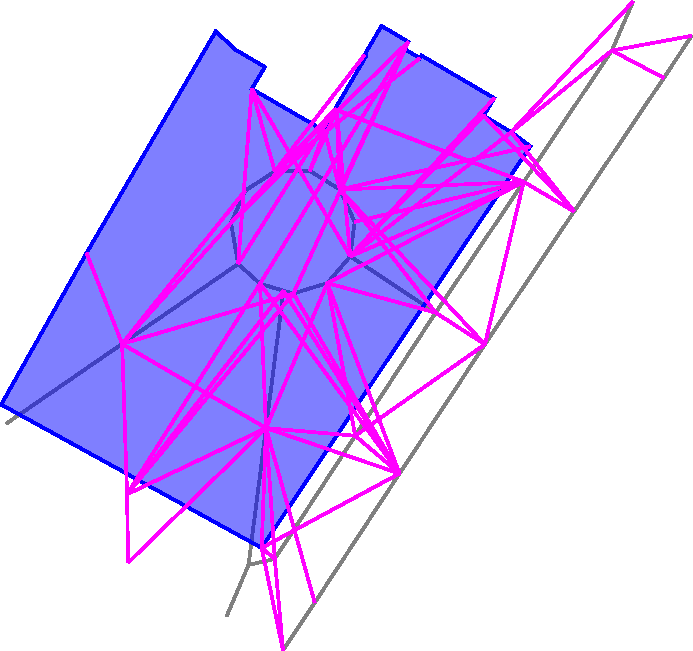
\includegraphics{../img/spojky.pdf}
	\caption{Spojky na malém území. Pokud bychom zde nevybírali náhodně, získali
	bychom velké množství spojek, které by zkrácení trasy příliš nepomohly.
	Růžové úsečky značí vytvořené spojky po náhodném výběru.}
	\label{fig:spojky}
\end{figure}

Spojky navíc mohou vést přes nějakou překážku, jako je plot nebo zeď, proto
potřebujeme zkontrolovat kolize všech přidaných spojek s~překážkami. K~tomuto
účelu jsme využili algoritmus využívající zametání roviny.


{\tuc Zametání roviny} \cite{zametani} je způsob návrhu geometrického algoritmu,
při němž rovinou posouváme přímku (\uv{zametáme}). Pokud přímka protne pro nás
zajímavé místo, vyvoláme událost. Během procházení si obvykle navíc pamatujeme
seznam prošlých bodů nebo aktuálně protnutých úseček, tzv. {\tuc průřez}.

V~našem případě budeme hledat průsečíky úseček v~rovině. Spojky již úsečky jsou,
překážky rozdělíme na jednotlivé úsečky mezi uzly. Budeme zametat podle od
západu k východu a zajímat nás budou události začátku a konce úsečky a jejich
průsečík. Zametací přímku proto budeme posouvat postupně po těchto událostech.

Začátky a konce úseček známe již před spuštěním algoritmu. Průsečíky na začátku
neznáme, budeme ale předpokládat, že se neprotínají tři úsečky v jednom bodě.
Potom platí, že pokud se nějaké dvě úsečky mají protnout, pak se předtím musí
stát sousedními. Proto nám stačí při každé události s úsečkou $u$ stačí
zkontrolovat sousedy $u$ a pokud se s nějakým protíná a průsečík je před
zametací přímkou, přidáme ho do seznamu událostí.

\begin{figure}[h]
	\centering
	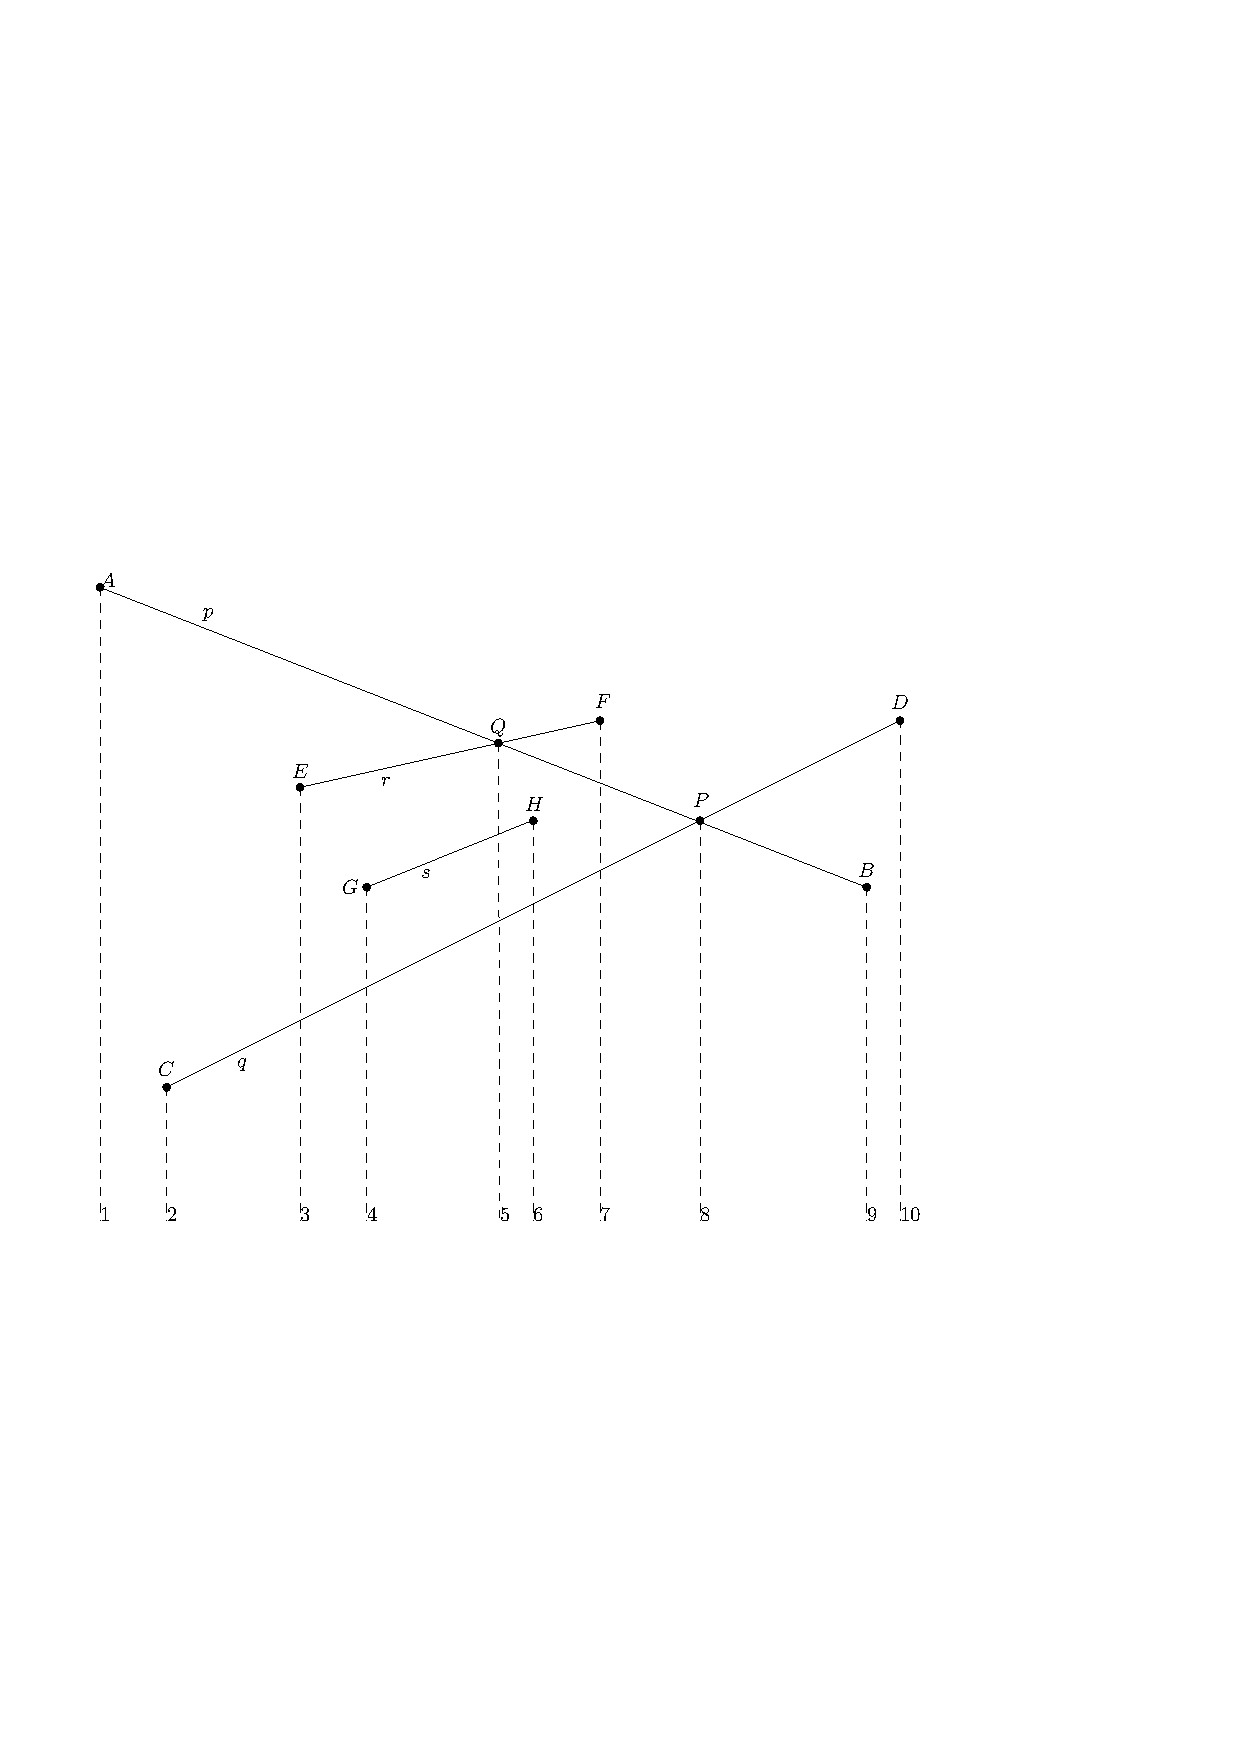
\includegraphics{../img/zametani.pdf}
	\caption{Zametání roviny}
	\label{fig:zametani}
\end{figure}

Protože vždy budeme potřebovat znát nejbližší událost, budeme si udržovat
události v~haldě. Dále také potřebujeme znát pořadí, v~jakém aktuálně
zpracovávané úsečky protínají rovinu -- průřez, a umět mezi ně přidat další a
odebrat tu, která skončí. K~tomuto účelu se nám hodí použít vyhledávací strom.
Nemůžeme si ovšem ve vrcholech pamatovat přímo souřadnice průsečíku úsečky se
zametací přímkou, protože se tyto souřadnice mění s~každým posunutím zametací
přímky. Místo toho si budeme ve stromě pamatovat jen odkazy na úsečky a průsečíky
budeme počítat, až to bude potřeba.

Na začátku známe všechny začátky a konce úseček, vytvoříme tedy v~haldě události
začátků a konců úseček. Průsečíkové události zatím žádné neznáme, ale protože
aby mohl nastat průsečík, musí nejprve úsečka začít, o~žádný nepřijdeme.

Zametání ukázkových dat se čtyřmi úsečkami ukazuje obrázek \ref{fig:zametani}.
Svislé přerušované čáry udávají pozice zametací přímky při vyvolání události,
události nastávají v pořadí 1 až 10.

Zametání bude probíhat následovně. Z~haldy všech událostí vybereme nejbližší
událost a rozhodneme se podle jejího typu:
\begin{itemize}
	\item {\tuc Začátek úsečky.}  Úsečku zařadíme na správné místo do
	průřezu a přidáme případné průsečíkové události se sousedními
	úsečkami.\\
	V situacích 1 a 4 úsečku pouze přidáme, k průsečíkům nedochází.\\
	V situacích 2 a 3 se úsečky protínají, přidáme průsečíkové události
	$P$ a $Q$.

	\item {\tuc Konec úsečky.} Úsečku odebereme z~průřezu a přidáme
	případnou průsečíkovou událost, pokud se úsečky sousední s~právě
	končící protínají.\\
	V situacích 7, 9 a 10 pouze úsečky odebereme z průřezu.\\
	V situaci 6 se po skončení úsečky $s$ stanou úsečky $p$ a $q$ sousedními
	a navíc se protínají, proto přidáme průsečíkovou událost $P$.
	\item {\tuc Průsečík úseček.} Úsečky v~průřezu prohodíme a přidáme
	případné průsečíkové události s~novými sousedy obou prohazovaných 
	úseček. Pokud jsme již průsečík těchto dvou úseček zpracovávali, událost
	zahodíme, protože úsečky se mohou protnout nejvýše jednou a další události
	jsou pouze násobným přidáním téže události (jako zde průsečíku $P$).\\
	V situaci 8 nemají prohozené úsečky žádné nové sousedy.\\
	V situaci 5 se nově stala úsečka $s$ sousedem prohozené přímky $p$, ale
	nemají společný průsečík, událost tedy nepřidáváme.
\end{itemize}
Takto budeme postupovat, dokud jsou v haldě nějaké události. Pokud zpracováváme 
průsečíkovou událost, zkontrolujeme, zda není některá z~úseček překážka a 
případně úsečky označíme, že se protnuly s~překážkou. 


\section{Zkratky přes průchozí prostranství}
Pokud procházíme ve městě přes větší park nebo náměstí, často nemusíme chodit
jen po chodnících, ale můžeme projít přes prostranství přímo. Přímé cesty přes
průchozí prostranství proto také chceme zanést do vyhledávacího grafu. K~jejich
vytvoření jsme využili modifikovaný algoritmus vytváření spojek mezi cestami.
Dvojice bodů v~průchozích prostranstvích jsme spojovali úsečkami. Tentokrát jsme
ale hledali dvojice bližší než 300 m, protože parky mohou být poměrně rozlehlé.
Opět jsme nepoužívali všechny dvojice ale jen některé náhodně vybrané, protože
jinak vznikalo příliš mnoho úseček, které vedly podobně, a proto nepřinášely
významné zlepšení vyhledané trasy. Protože i na průchozích prostranstvích se
vyskytují překážky, opět jsme pomocí zametání roviny odstranili všechny úsečky,
které procházely přes nějakou překážku.

\section{Vytvoření vyhledávacího grafu}
Poté, co jsme připravili data, vytvoříme vyhledávací graf. Protože kolize
přímých cest s~překážkami jsme vyřešili již při jejich vytváření, jsou všechny
cesty korektní. Proto se překážkami již dále nezabýváme a pouze z~cest vytvoříme
vyhledávací graf. Pokud byly v datech přítomny cesty nepřipojené ke zbytku a ani 
přidání spojek a zkratek je nepřipojilo, měl by tento graf více komponent. Tyto
převážně malé komponenty nás nezajímají, protože do nich neumíme najít cestu, a
proto použijeme jen největší komponentu. Uložíme seznam všech uzlů, které jsou
na jejích cestách použity a cesty rozdělíme na jednotlivé hrany grafu mezi dvěma
uzly.  U~hran zachováme údaje o~typu cesty, protože je budeme využívat při
vyhledávání.


% Ukázka použití některých konstrukcí LateXu (odkomentujte, chcete-li)
% \include{ukazka}

\chapter*{Závěr}
\addcontentsline{toc}{chapter}{Závěr}

zrychleni - potencialova heuristika, viz MJ - skripta z GA

skriptovani vypoctu penalt

Další možné rozšíření systému penalt by mohlo být například posuzování intervalů
linek, kdy bychom mohli preferovat častěji jedoucí linky. 

posun odchodu podle prvniho MHD

okolí cest


%%% Seznam použité literatury
\def\bibname{Seznam použité literatury}
%%% Seznam použité literatury je zpracován podle platných standardů. Povinnou citační
%%% normou pro bakalářskou práci je ISO 690. Jména časopisů lze uvádět zkráceně, ale jen
%%% v kodifikované podobě. Všechny použité zdroje a prameny musí být řádně citovány.

\def\bibname{Seznam použité literatury}
\begin{thebibliography}{99}
\addcontentsline{toc}{chapter}{\bibname}

\bibitem{lamport94}
  {\sc Lamport,} Leslie.
  \emph{\LaTeX: A~Document Preparation System}.
  2. vydání.
  Massachusetts: Addison Wesley, 1994.
  ISBN 0-201-52983-1.

\bibitem{osmweb}
	\emph{OpenStreetMap} [online]. 
	2014, 4.5.2014 [cit. 2014-05-04]. 
	Dostupné z: \url{http://www.openstreetmap.org}

\bibitem{osmxml}
	\emph{OSM XML} [online]. 
	2014, 16 September 2013 [cit. 2014-05-06]. 
	Dostupné z: \url{http://wiki.openstreetmap.org/wiki/OSM_XML}

\bibitem{osmfeatures}
	\emph{Cs: Map Features} [online]. 
	2014-04-01 [cit. 2014-05-17]. 
	Dostupné z: \url{http://wiki.openstreetmap.org/wiki/Cs:Map_Features}

\bibitem{wgsnorma}
	{\sc NIMA.}
	\emph{World geodetic system 1984} [online]. 
	3. vydání, 1. dodatek.
	3 January 2000 [cit. 2014-05-04]. 
	Dostupné z: \url{http://www2.jpl.nasa.gov/srtm/}.

\bibitem{utmnorma}
	{\sc Snyder,} John P.
	\emph{Map Projections: A~Working Manual} [online]. 
	1987, [cit. 2014-05-08]. 
	Dostupné z: \url{http://pubs.er.usgs.gov/publication/pp1395}.

\bibitem{srtmweb}
	{\sc NASA.}
	\emph{The Shuttle Radar Topography Mission} [online]. 
	2014, June 17, 2009 [cit. 2014-05-04]. 
	Dostupné z: \url{http://www2.jpl.nasa.gov/srtm/}.

\bibitem{pbfweb}
	{\sc Google.}
	\emph{Protocol Buffers} [online]. 
	2014, April 2, 2012 [cit. 2014-05-05]. 
	Dostupné z: \url{https://developers.google.com/protocol-buffers/}.

\bibitem{pbfenc}
	{\sc Google.}
	\emph{Encoding - Protocol Buffers} [online]. 
	2014, April 2, 2012 [cit. 2014-05-07]. 
	Dostupné z: \url{https://developers.google.com/protocol-buffers/docs/encoding}.

\bibitem{pbfspec}
	{\sc Google.}
	\emph{Language Guide - Protocol Buffers} [online]. 
	2014, April 22, 2014 [cit. 2014-05-07]. 
	Dostupné z:	\url{https://developers.google.com/protocol-buffers/docs/proto}.

\bibitem{lineint}
	{\sc Weisstein} Eric W.
	\emph{Line-Line Intersection.} [online]. 
	2014, May 12, 2014 [cit. 2014-05-12]. 
	Dostupné z:	\url{http://mathworld.wolfram.com/Line-LineIntersection.html}.

\bibitem{zametani}
	{\sc Mareš} Martin
	\emph{Geometrické algortimy} [online]. 
	2014, 17.11.2013 [cit. 2014-05-13]. 
	Dostupné z:	\url{http://mj.ucw.cz/vyuka/ads/43-geom.pdf}.
	

\end{thebibliography}



%%% Tabulky v bakalářské práci, existují-li.
\chapwithtoc{Seznam tabulek}

%%% Použité zkratky v bakalářské práci, existují-li, včetně jejich vysvětlení.
\chapwithtoc{Seznam použitých zkratek}

%%% Přílohy k bakalářské práci, existují-li (různé dodatky jako výpisy programů,
%%% diagramy apod.). Každá příloha musí být alespoň jednou odkazována z vlastního
%%% textu práce. Přílohy se číslují.
\chapwithtoc{Přílohy}

\openright
\end{document}
